\documentclass[UTF8]{ctexart}
\usepackage{mathtools}
\usepackage{amsmath}
\usepackage{listings}
\usepackage{fancybox}
\usepackage{xcolor}
\usepackage{rotating}
\usepackage{diagbox}
\usepackage{amssymb}
\usepackage{warpcol}
\usepackage{lscape}
\usepackage[framemethod=tikz]{mdframed}
\usepackage{longtable,booktabs}
\usepackage{bm}

\definecolor{ocre}{RGB}{243,102,25}
\definecolor{mygray}{RGB}{243,243,244}


\lstset{
columns=flexible,
numbers=left,
numberstyle=\footnotesize\color{darkgray}, 
basicstyle=\small\ttfamily,
stringstyle=\color{purple},
keywordstyle=\color[RGB]{40,40,255}\bfseries,
commentstyle=\it\color[RGB]{0,96,96},  
stringstyle=\rmfamily\slshape\color[RGB]{128,0,0}, 
showstringspaces=false,      
% directivestyle=\color{blue},
frame=shadowbox,
%framerule=0pt,
backgroundcolor=\color[RGB]{245,245,244},
escapeinside=``, %逃逸字符(1左面的键),用于显示中文
breaklines,
extendedchars=false,
%解决代码跨页时,章节标题,页眉等汉字不显示的问题
xleftmargin=2em,xrightmargin=2em,
aboveskip=1em,%设置边距
tabsize=4, %设置tab空格数  
showspaces=false %不显示空格 
rulesepcolor=\color{red!20!green!20!blue!20}
%rulesepcolor=\color{brown}
}

\title{\heiti 多商品流问题及数值实验}
\author{\kaishu 张晋\\
				\kaishu 北京航空航天大学,数学与系统科学学院}
\date{\today}
\begin{document}
\maketitle
\newpage
\section{引言}
    {\enspace}{
多商品流问题(MultiCommodity Flow Problem, MCFP)是多种物品在网络中从不同的源点流向不同的汇点的网络流问题。
}

\section{多商品网络流模型}
已知一有向网络 $\mathcal{G}=(\mathcal{N},\mathcal{E})$,
其中 $\mathcal{N}$ 是节点集, $\mathcal{E}$ 是弧集. 
对每条弧 $l = (i, j) \in \mathcal{E} $,
设其容量是 $c_l$ , 代表每条弧上所能承受负载的上界.

已知有$M$ 件物品 $K_{1},K_{2},\dots ,K_{M}$,
定义为$K_{m}=(s_{m},t_{m},d_{m}) $,
其中$ s_{m}$ 和$t_{m}$ 是物品${m}$的源点及汇点,$ d_{m}$是流量需求,这代表流量在节点$s_m$流入网络,然后在节点$t_m$流出网络, $d_m$代表物品$m$流出减流入的量。

我们设物品$m$沿弧 $l$的流量是$f_{ml} $,
则该流量分配需要满足以下条件:

a)容量约束:
\begin{equation}
f_l=\sum_{m=1}^{M} f_{ml} \leq c_l\quad \forall l \in\mathcal{E} 
\end{equation}

b)流平衡约束:
\begin{equation}
\sum_{l:l=(i,j)\in \mathcal{E}} f_{ml} -\sum_{l:l=(j,i)\in \mathcal{E}} f_{ml}
=b_{mi}=
\begin{dcases}  
0,& i \neq s_m,t_m\\
d_m,& i=s_m\\
-d_m,& i=t_m
\end{dcases}
\end{equation}

c)流非负:
\begin{equation}
f_{ml}\geq 0,\quad m=1,\cdots,M,\forall l \in \mathcal{E}
\end{equation}


令$\bm{A}$是网络$\mathcal{G}$ 的点弧关联矩阵,
即$N \times E$ 阶矩阵,且第 $l$列与弧$l = (i, j)$对
应,仅第$i$行的元素为1,第$ j$行的元素为−1 ,
其余元素为0. 再令$ \bm{b}_m=(b_{m1},\cdots,
b_{mN})^{T}, \bm{f}_m=(f_{m1},\ f_{m2}, \cdots,\ f_{mE})^T$,
则可将等式约束(2)表示成
\[\bm{A}\bm{f}_m=\bm{b}_m\]

\newpage
\section{最优流量工程}
若存在流分布$\bm{f}$满足流量约束,
我们应该思考怎样改变$\bm{f}$使得在其满足流量约束条件的同时,
每条弧的利用率都不高,也就是说尽量避免某条弧堵塞的情况。

对此我们可以给定一个成本函数$\phi(\bm{f})$来评价整体网络的堵塞情况,这里$\phi(\bm{f})$是$\bm{f}$的非减函数。最优流量工程即意味着在满足多商品流约束条件下,使得成本函数$\phi(\bm{f})$取得极小值,那么多商品流问题可转化为解决一个线性规划问题:
\begin{alignat}{2}
min \quad & \phi(\bm{f},\bm{c})&{}\\
\mbox{s.t.}\quad
&\bm{f}=\sum_{m=1}^M \bm{f}_m&{} \\
&\bm{A}\bm{f}_m=\bm{b}_m,\quad &m=1,\cdots,M\\
&\bm{f}_m \geq \bm{0},&m=1,\cdots,M
\end{alignat}

在所有关于流量工程的论文中, 最大弧利用
率(Maximum Arc Utilization, MAU) 和 M/M/1 延迟
公式的逐段线性近似是两个使用最多的成本函数

极小化MAU确保最拥塞的热点弧利用率尽可能的小,这里的MLU可以用
弧上的负载和容量表述为
\begin{equation}
\phi(\bm{f})=\max\limits_{l \in \mathcal{E}}f_l/c_l
\end{equation}


基于该目标函数的多商品流问题可转化为以下线性规划:


\begin{alignat}{2}
\mbox{minimize}\quad &z&{} \nonumber\\
\mbox{subject to}\quad &
\sum_{m=1}^M f_{ml}/c_l-z\leq 0,\quad&\forall l\in \mathcal{E} \nonumber\\
&\bm{A}\bm{f}_m=\bm{b}_m,\quad &m=1,\cdots,M\nonumber\\
&\bm{f}_m \geq \bm{0},&m=1,\cdots,M
\end{alignat}

\newpage
M/M/1延迟公式的逐段线性近似由 Fortz 等提
出,是经作者与贝尔实验室的技术人员讨论后
得到的. 下面将它简称它为 FT 成本函数,
可以将 FT 成本函数表述为$\phi(\bm{f})=\sum_{l \in \mathcal{E}}\phi(f_l)$,其中

\begin{equation}
\varphi(f_{l})=\left\{\begin{array}{ll}
f_{l},& \frac{f_{l}}{c_{l}}\leq\frac{1}{3}\\
3f_{l}-\frac{2}{3}c_{l},& \frac{1}{3}<\frac{f_l}{c_{l}}\leq\frac{2}{3}\\
10f_{l}-\frac{16}{3}c_{l},& \frac{2}{3}<\frac{f_l}{c_{l}}\leq\frac{9}{10}\\
70\ f_{l}-\frac{178}{3}c_{l},& \frac{9}{10}<\frac{f_{l}}{c_{l}}\leq 1\\
500f_{l}-\frac{1468}{3}c_{l},& 1<\frac{f_{l}}{c_{l}}\leq\frac{11}{10}\\
5000\ f_{l}-\frac{16318}{3}c_{l},& \frac{11}{10}<\frac{f_l}{c_{l}}<\infty
\end{array}\right.
\end{equation}

基于 FT 成本函数的多商品流问题也可转化为线性规划问题:
\begin{alignat}{2}
\mbox{minimize}\quad &\sum_{l \in \mathcal{E}}z_l&{}\nonumber\\
\mbox{subject to}\quad &
\sum_{m} f_{ml}-z_l\leq 0,\quad&\forall l\in \mathcal{E} \nonumber\\
&3\sum_{m} f_{ml}-z_l\leq \frac{2}{3}c_{l},\quad&\forall l\in \mathcal{E} \nonumber\\
&10\sum_{m} f_{ml}-z_l\leq \frac{16}{3}c_{l},\quad&\forall l\in \mathcal{E} \nonumber\\
&70\sum_{m} f_{ml}-z_l\leq \frac{178}{3}c_{l},\quad&\forall l\in \mathcal{E} \nonumber\\
&500\sum_{m} f_{ml}-z_l\leq \frac{1468}{3}c_{l},\quad&\forall l\in \mathcal{E} \nonumber\\
&5000\sum_{m} f_{ml}-z_l\leq \frac{16318}{3}c_{l},\quad&\forall l\in \mathcal{E} \nonumber\\
&\bm{A}\bm{f}_m=\bm{b}_m,\quad &m=1,\cdots,M\nonumber\\
&\bm{f}_m \geq \bm{0},&m=1,\cdots,M
\end{alignat}

\newpage
\section{数值实验}
我们先来看TE中的一个经典例子,这个网络有7个节点13条弧,每条弧的容量是5个单位. 此外有四个
需求量均为4个单位的源—目的对$(M =4)$,具体
的源节点、目的节点信息如图如图\ref{fig:1}所示.表1为点弧关联矩阵。这里为了简单,
省去了未用到的弧. 此外,弧上的数字表示弧的编
号,此时$\bm{c}^T=(5,5,\cdots,5)_{1\times 13}$


\begin{figure}[h]
\small
\centering
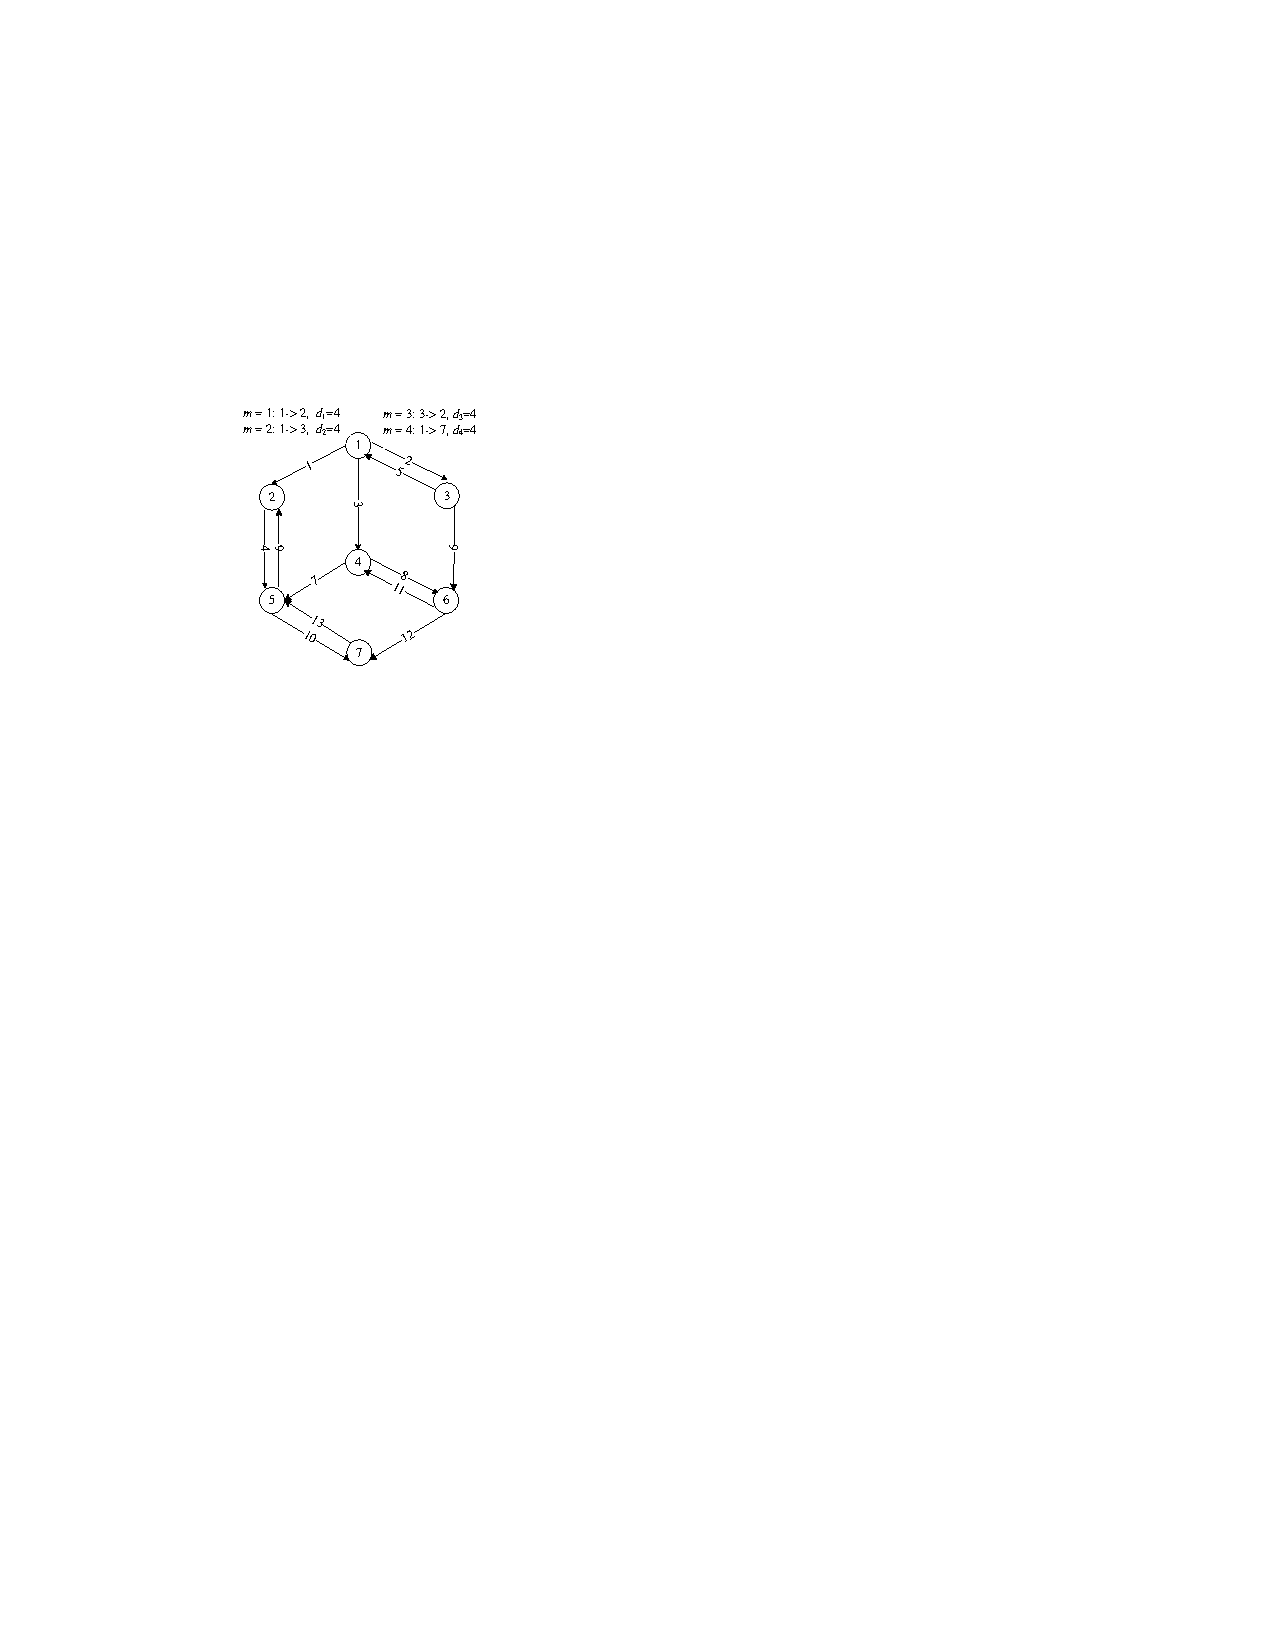
\includegraphics[width=8cm]{f1.pdf}
\caption{经典例子}
\label{fig:1}
\end{figure}


\[\bm{b}_1=\begin{bmatrix}
4\\-4\\0\\0\\0\\0\\0
\end{bmatrix},\qquad
\bm{b}_2=\begin{bmatrix}
4\\0\\-4\\0\\0\\0\\0
\end{bmatrix},\qquad
\bm{b}_3=\begin{bmatrix}
0\\-4\\4\\0\\0\\0\\0
\end{bmatrix},\qquad
\bm{b}_4=\begin{bmatrix}
4\\0\\0\\0\\0\\0\\-4
\end{bmatrix}
\]
\begin{table}[htbp]
\centering
\label{e1}

\[\bm{A}_1 = \left[ {\begin{array}{*{20}{c}}
1&1&1&{}&-1&{}&{}&{}&{}&{}&{}&{}&{}\\
-1&{}&{}&1&{}&{}&{}&{}&-1&{}&{}&{}&{}\\
{}&-1&{}&{}&1&1&{}&{}&{}&{}&{}&{}&{}\\
{}&{}&-1&{}&{}&{}&1&1&{}&{}&-1&{}&{}\\
{}&{}&{}&-1&{}&{}&-1&{}&1&1&{}&{}&-1\\
{}&{}&{}&{}&{}&-1&{}&-1&{}&{}&1&1&{}\\
{}&{}&{}&{}&{}&{}&{}&{}&{}&-1&{}&-1&1
\end{array}} \right]\]
\caption{点弧关联矩阵}
\end{table}

\newpage
在此我们对该例子进行数值实验,考虑到MATLAB线性规划函数linprog的自变量只能为向量,我们需要对原线性规划进行变形,变成如下形式:

\begin{alignat}{2}
\mbox{minimize}\quad &\bm{f}^T\bm{x} \nonumber\\
&\bm{A}\cdot\bm{x}\leq\bm{b}\nonumber\\
&Aeq\cdot\bm{x}=beq\nonumber\\
&lb\leq \bm{x}\leq ub
\end{alignat}

\newpage
\subsection{MAU}
在使用MAU方法时,需进行以下变形:
\[\bm{x}=\begin{bmatrix}
\bm{f}_{1l}\\\bm{f}_{2l}\\\bm{f}_{3l}\\\bm{f}_{4l}\\z
\end{bmatrix}_{53\times 1},\qquad
\bm{f}_{il}=\begin{bmatrix}
f_{i1}\\f_{i2}\\f_{i3}\\ \vdots\\ f_{i13}
\end{bmatrix}_{13\times 1},\qquad
\bm{f}=\begin{bmatrix}
0\\0\\ \vdots\\0\\ 1
\end{bmatrix}_{53\times 1},\qquad
\bm{f}^T\bm{x}=z\]

\[\bm{A}=\begin{bmatrix}
\bm{I},&\bm{I},&\bm{I},&\bm{I},&-\bm{c}
\end{bmatrix}_{13\times 53},\qquad
\bm{A}\cdot\bm{x}=\bm{f}_{1l}+\bm{f}_{2l}+\bm{f}_{3l}+\bm{f}_{4l}-z\cdot \bm{c}
\]
其中$\bm{I}$是$13\times 13$的单位向量,$\bm{b}$为$13\times 1$的零向量.

\[Aeq=\begin{bmatrix}
\bm{A}_1&{}&{}&{}&\bm{0}\\
{}&\bm{A}_1&{}&{}&\bm{0}\\
{}&{}&\bm{A}_1&{}&\bm{0}\\
{}&{}&{}&\bm{A}_1&\bm{0}
\end{bmatrix}_{28\times 53}\]

\[
Aeq\cdot \bm{x}=\begin{bmatrix}
\bm{A}_1&{}&{}&{}&\bm{0}\\
{}&\bm{A}_1&{}&{}&\bm{0}\\
{}&{}&\bm{A}_1&{}&\bm{0}\\
{}&{}&{}&\bm{A}_1&\bm{0}
\end{bmatrix}\cdot
\begin{bmatrix}
\bm{f}_{1l}\\\bm{f}_{2l}\\\bm{f}_{3l}\\\bm{f}_{4l}\\z
\end{bmatrix}=
\begin{bmatrix}
\bm{A}_1\bm{f}_{1l}\\
\bm{A}_1\bm{f}_{2l}\\
\bm{A}_1\bm{f}_{3l}\\
\bm{A}_1\bm{f}_{4l}
\end{bmatrix}=
\begin{bmatrix}
\bm{b}_1\\\bm{b}_2\\\bm{b}_3\\\bm{b}_4
\end{bmatrix}_{28\times 1}=beq\]
$\bm{lb}$为$53\times 1$的零向量,$ub$为空.

\newpage
\subsection{M/M/1}
在对M/M/1延迟公式进行计算时,需要进行以下变形:
\[\bm{x}=\begin{bmatrix}
\bm{f}_{1l}\\\bm{f}_{2l}\\\bm{f}_{3l}\\\bm{f}_{4l}\\\bm{z}_{l}
\end{bmatrix}_{65\times 1},\qquad
\bm{z}_{l}=\begin{bmatrix}
z_{1}\\z_{2}\\z_{3}\\ \vdots\\ z_{13}
\end{bmatrix}_{13\times 1},\qquad
\bm{f}=\begin{bmatrix}
0\\0\\ \vdots\\1\\ 1
\end{bmatrix}_{(52+13)\times 1},\qquad
\bm{f}^T\bm{x}=\sum_{l \in \mathcal{E}}z_l\]

\[\bm{A}=\begin{bmatrix}
\bm{I},&\bm{I},&\bm{I},&\bm{I},&-\bm{I}\\
3\bm{I},&3\bm{I},&3\bm{I},&3\bm{I},&-\bm{I}\\
10\bm{I},&10\bm{I},&10\bm{I},&10\bm{I},&-\bm{I}\\
70\bm{I},&70\bm{I},&70\bm{I},&70\bm{I},&-\bm{I}\\
500\bm{I},&500\bm{I},&500\bm{I},&500\bm{I},&-\bm{I}\\
5000\bm{I},&5000\bm{I},&5000\bm{I},&5000\bm{I},&-\bm{I}\\
\end{bmatrix}_{78\times 65},\qquad
\bm{b}=\begin{bmatrix}
\bm{0}\\
\frac{2}{3}\bm{c}_l\\
\frac{16}{3}\bm{c}_l\\
\frac{178}{3}\bm{c}_l\\
\frac{1468}{3}\bm{c}_l\\
\frac{16318}{3}\bm{c}_l
\end{bmatrix}_{78\times 1}
\]
其中$\bm{I}$是$13\times 13$的单位向量.
\[Aeq=\begin{bmatrix}
\bm{A}_1&{}&{}&{}&\bm{0}\\
{}&\bm{A}_1&{}&{}&\bm{0}\\
{}&{}&\bm{A}_1&{}&\bm{0}\\
{}&{}&{}&\bm{A}_1&\bm{0}
\end{bmatrix}_{28\times 65}\]
\[
Aeq\cdot \bm{x}=\begin{bmatrix}
\bm{A}_1&{}&{}&{}&\bm{0}\\
{}&\bm{A}_1&{}&{}&\bm{0}\\
{}&{}&\bm{A}_1&{}&\bm{0}\\
{}&{}&{}&\bm{A}_1&\bm{0}
\end{bmatrix}\cdot
\begin{bmatrix}
\bm{f}_{1l}\\\bm{f}_{2l}\\\bm{f}_{3l}\\\bm{f}_{4l}\\\bm{z}_{l}
\end{bmatrix}=
\begin{bmatrix}
\bm{A}_1\bm{f}_{1l}\\
\bm{A}_1\bm{f}_{2l}\\
\bm{A}_1\bm{f}_{3l}\\
\bm{A}_1\bm{f}_{4l}
\end{bmatrix}=
\begin{bmatrix}
\bm{b}_1\\\bm{b}_2\\\bm{b}_3\\\bm{b}_4
\end{bmatrix}_{28\times 1}=beq\]

$\bm{lb}$为$65\times 1$的零向量,$ub$为空.

\newpage
\section{MATLAB程序及运行结果}
\begin{lstlisting}[language=Octave]
%MAU
f=[zeros(52,1);1];
A=[1,1,1,0,-1,0,0,0,0,0,0,0,0;
  -1,0,0,1,0,0,0,0,-1,0,0,0,0;
   0,-1,0,0,1,1,0,0,0,0,0,0,0;
   0,0,-1,0,0,0,1,1,0,0,-1,0,0;
   0,0,0,-1,0,0,-1,0,1,1,0,0,-1;
   0,0,0,0,0,-1,0,-1,0,0,1,1,0;
   0,0,0,0,0,0,0,0,0,-1,0,-1,1];
Aeq=[blkdiag(A,A,A,A),zeros(28,1)];
b1=[4,-4,0,0,0,0,0]';
b2=[4,0,-4,0,0,0,0]';
b3=[0,-4,4,0,0,0,0]';
b4=[4,0,0,0,0,0,-4]';
beq=[b1;b2;b3;b4];
I=eye(13);
c=5*ones(13,1);
a=[I,I,I,I,-c];
b=zeros(13,1);
lb=zeros(53,1);
x=linprog(f,a,b,Aeq,beq,lb,[]);
F=[x(1:13,:)';
   x(14:26,:)';
   x(27:39,:)';
   x(40:52,:)']
\end{lstlisting}

程序运行结果如下:
\[\bm{f}= (f_{ml})_{4\times 13}=\left[ {\begin{array}{*{20}{c}}
4&0&0&0&0&0&0&0&0&0&0&0&0\\
0&4&0&0&0&0&0&0&0&0&0&0&0\\
0&0&0&0&0&4&0&0&4&0&0&4&4\\
0&0&4&0&0&0&4&0&0&4&0&0&0
\end{array}} \right]\]

\[\qquad \phi(\bm{f})=0.8\]


\newpage
\begin{lstlisting}[language=Octave]
%M/M/1
f=[zeros(52,1);ones(13,1)];
A=[1,1,1,0,-1,0,0,0,0,0,0,0,0;
  -1,0,0,1,0,0,0,0,-1,0,0,0,0;
   0,-1,0,0,1,1,0,0,0,0,0,0,0;
   0,0,-1,0,0,0,1,1,0,0,-1,0,0;
   0,0,0,-1,0,0,-1,0,1,1,0,0,-1;
   0,0,0,0,0,-1,0,-1,0,0,1,1,0;
   0,0,0,0,0,0,0,0,0,-1,0,-1,1];
Aeq=[blkdiag(A,A,A,A),zeros(28,13)];
b1=[4,-4,0,0,0,0,0]';
b2=[4,0,-4,0,0,0,0]';
b3=[0,-4,4,0,0,0,0]';
b4=[4,0,0,0,0,0,-4]';
beq=[b1;b2;b3;b4];
I=eye(13);
T=[I;3*I;10*I;70*I;500*I;5000*I];
i=-[I;I;I;I;I;I];
a=[T,T,T,T,i];
c=5*ones(13,1);
b=[0*c;2/3*c;16/3*c;178/3*c;1468/3*c;16318/3*c];
lb=zeros(65,1);
x=linprog(f,a,b,Aeq,beq,lb,[]);
F=[x(1:13,:)';
   x(14:26,:)';
   x(27:39,:)';
   x(40:52,:)']
sum(x(53:end,:))
\end{lstlisting}
程序运行结果如下:

\[\bm{f}=\left[ {\begin{array}{*{20}{c}}
4&0&0&0&0&0&0&0&0&0&0&0&0\\
0&4&0&0&0&0&0&0&0&0&0&0&0\\
0.5&0&0.1667&0&0.6667&3.3333&1.8333&0&3.5&0&1.6667&1.6667&1.6667\\
0&0&4&0&0&0&2.3333&1.6667&0&2.3333&0&1.6667&0
\end{array}} \right]\]

\[\qquad \phi(\bm{f})=92.6667\]

\section{结果分析}
我们观察所得流分布矩阵,可以看出两种方案所得结果差异不是很大,
将MAU方案和M/M/1方案转移的总流量分别加起来,MAU方案共转移了36单位流量,而M/M/1方案转移了35单位流量,如果需要考虑转移流量的成本,M/M/1方案要更为优异。

而我们可以看出,M/M/1方案中的最大弧利用率也为0.8,这和MAU方案的结果相同,而MAU方案中的FT成本函数值显然要比M/M/1方案中大,从这两个角度来说,M/M/1方案都要比MAU方案好。

然而M/M/1方案中不等式约束更多,也需要花更多内存和时间来计算,在本例子中,MAU方案的线性不等式约束矩阵$\bm{A}$大小为$13\times 53$,而M/M/1方案的$\bm{A}$矩阵大小为$78\times 65$,差异约为6倍,该差异来源于FT函数中多出的6 个不等式,故在其他例子的测试中,该差异应该也会恒定在6倍左右。

综上,只考虑结果的优异性时,M/M/1方案从各个方面都更好,但在大规模的测试问题中,我们就要考虑到计算成本的因素,可以选择更省时省力的MAU方案。

\end{document}